\section{Data analysis}
\subsection{Introduction/Overview}
This section aims to quantitatively analyze and compare the performance of large language models (LLMs) in Java to C++ code translation tasks. By manually analyzing and annotating the types of hallucinations generated during the translation process, compiling statistics, and calculating the frequency of various errors, we further analyze the key factors influencing LLM performance. This provides empirical evidence for evaluating the current capabilities and limitations of LLMs in code project translation.

The dataset analyzed in this study is derived from the work of researchers who translated methods from 5-6 Java projects into C++ using different LLMs and methods. This dataset comprises a total of 1994 translated methods, which have undergone meticulous manual error type annotation.

We systematically explore LLM performance across three primary analytical dimensions to comprehensively understand translation efficiency and hallucination patterns:
\begin{itemize}[leftmargin=1.5em]
    \item \textbf{Model: }Compares the performance of GPT (representing widely adopted general-purpose LLMs) and DeepSeek (an emerging specialized or alternative LLM).
    \item \textbf{Error Type: }Employs a detailed, manually identified error classification scheme to categorize and annotate the most common errors occurring during the translation process by existing large language models. This aids in precisely understanding the common errors and concentration of LLM hallucinations.
\end{itemize}

\subsection{Statistical Methods}
The quantitative analysis in this study involves calculating metrics for evaluating LLM translation hallucinations: correctness rate and error rate, which are defined as the number of correctly and incorrectly translated methods divided by the total number of methods, respectively. These metrics were calculated for different groupings to facilitate further comparative analysis.

\subsection{Identified Errors}
To systematically quantify and analyze the "hallucination" phenomenon of large language models in Java to C++ code translation tasks, we established a detailed error classification standard. Through meticulous manual review of the translation results, we identified and summarized several core error types that repeatedly occurred during the translation process.

\subsubsection{Referencing non-existent methods or member variables}
This error type refers to calling a method in the translated code that does not exist in a class or its base class. This usually happens when the model attempts to directly migrate a specific API or programming habit from the source language to the target language, but the corresponding class library in the target language does not have a functionally equivalent member function.
\begin{figure}[H]
  \centering
  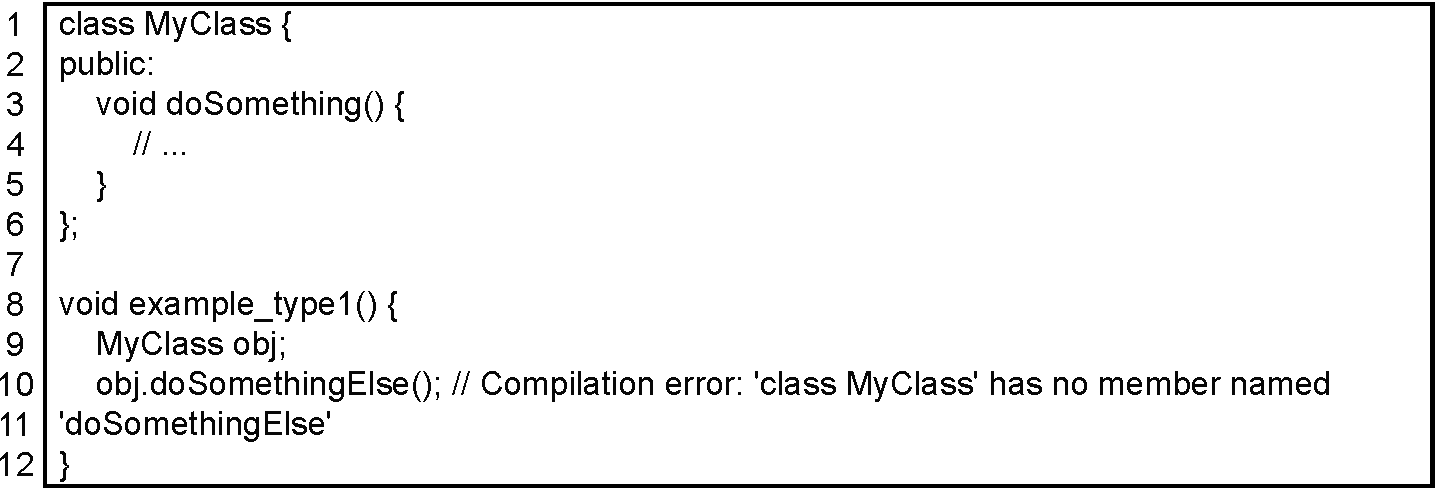
\includegraphics[width=0.5\textwidth]{pdf/Codes/Code1.pdf}
\end{figure}
\subsubsection{Parameter list mismatch}
When code calls a function or method, the provided parameters do not match the parameter list of any available overloaded version of that function in terms of quantity, type, or order.
\begin{figure}[H]
  \centering
  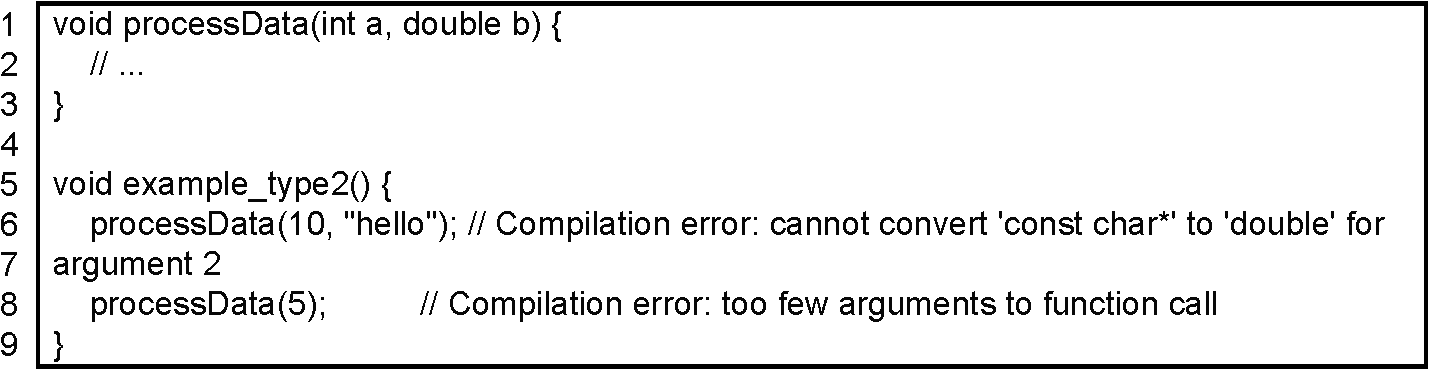
\includegraphics[width=0.5\textwidth]{pdf/Codes/Code2.pdf}
\end{figure}
\subsubsection{Missing header file}
The code uses a class, function, or macro defined in the C++ standard library or other parts of the project, but does not include the corresponding header file via an \#include directive, causing the compiler to fail to find the definition of related symbols, thus leading to compilation failure. This error needs to be distinguished from "Referencing non-existent classes": in type 3, the referenced symbol itself exists, only the declaration is missing; while in type 7, the referenced class is entirely fictitious.
\begin{figure}[H]
  \centering
  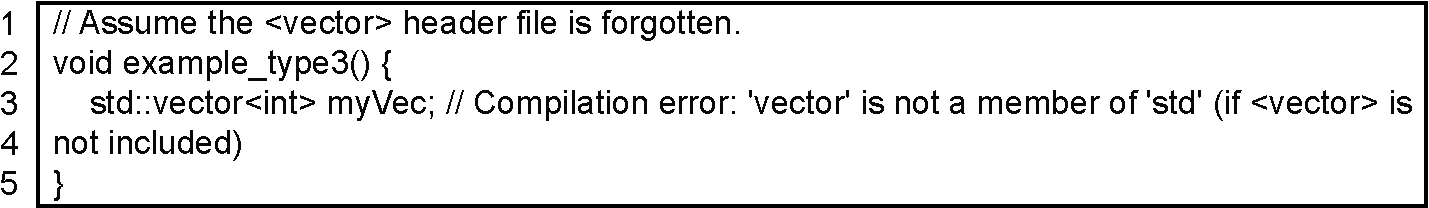
\includegraphics[width=0.5\textwidth]{pdf/Codes/Code3.pdf}
\end{figure}
\subsubsection{Method not implemented (entirely missing)}
This error type refers to a member function being declared in the class's header file or source file, but no implementation for that function is provided at all in the corresponding source file, or the implementation body is empty.
\begin{figure}[H]
  \centering
  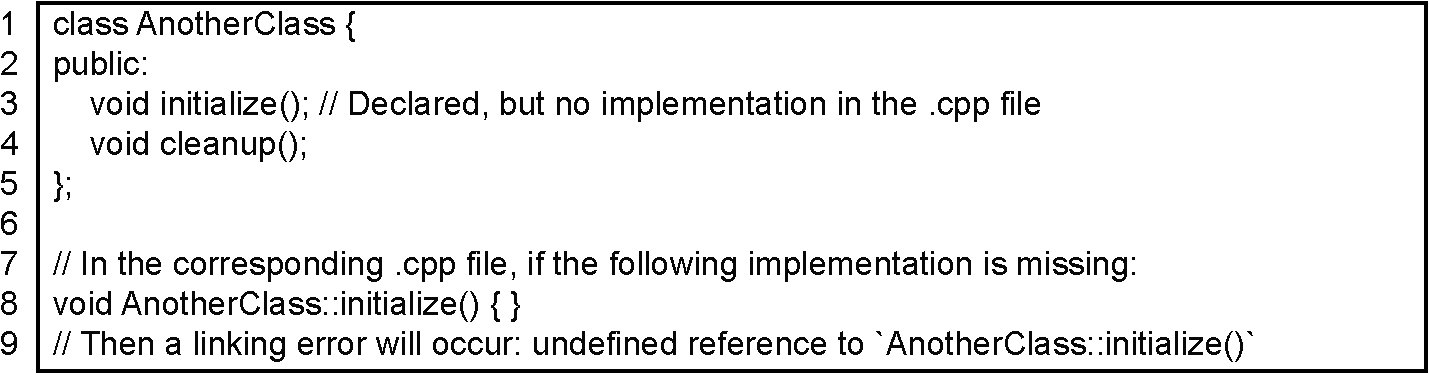
\includegraphics[width=0.5\textwidth]{pdf/Codes/Code4.pdf}
\end{figure}
\subsubsection{Variable initialization/usage error}
This error type typically includes not initializing reference members or constant members in the constructor's member initializer list. Additionally, using uninitialized variables also falls into this category.
\begin{figure}[H]
  \centering
  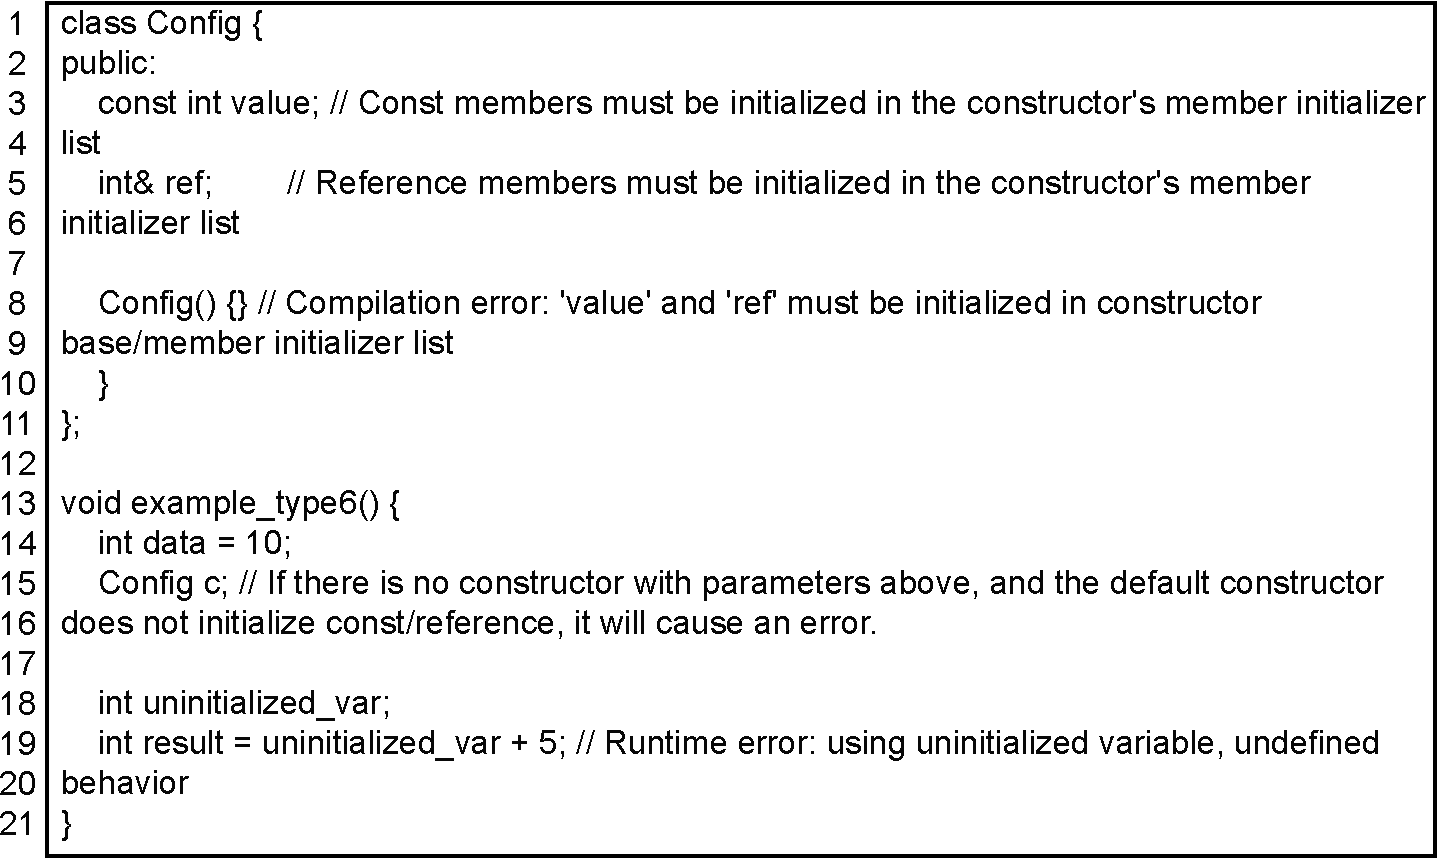
\includegraphics[width=0.5\textwidth]{pdf/Codes/Code5.pdf}
\end{figure}
\subsubsection{Incorrect pointer usage}
This error type involves improper operations on C++ pointers (including raw pointers and smart pointers). For example, dereferencing a void pointer and attempting to call its member method, or incorrectly performing pointer type conversions.
\begin{figure}[H]
  \centering
  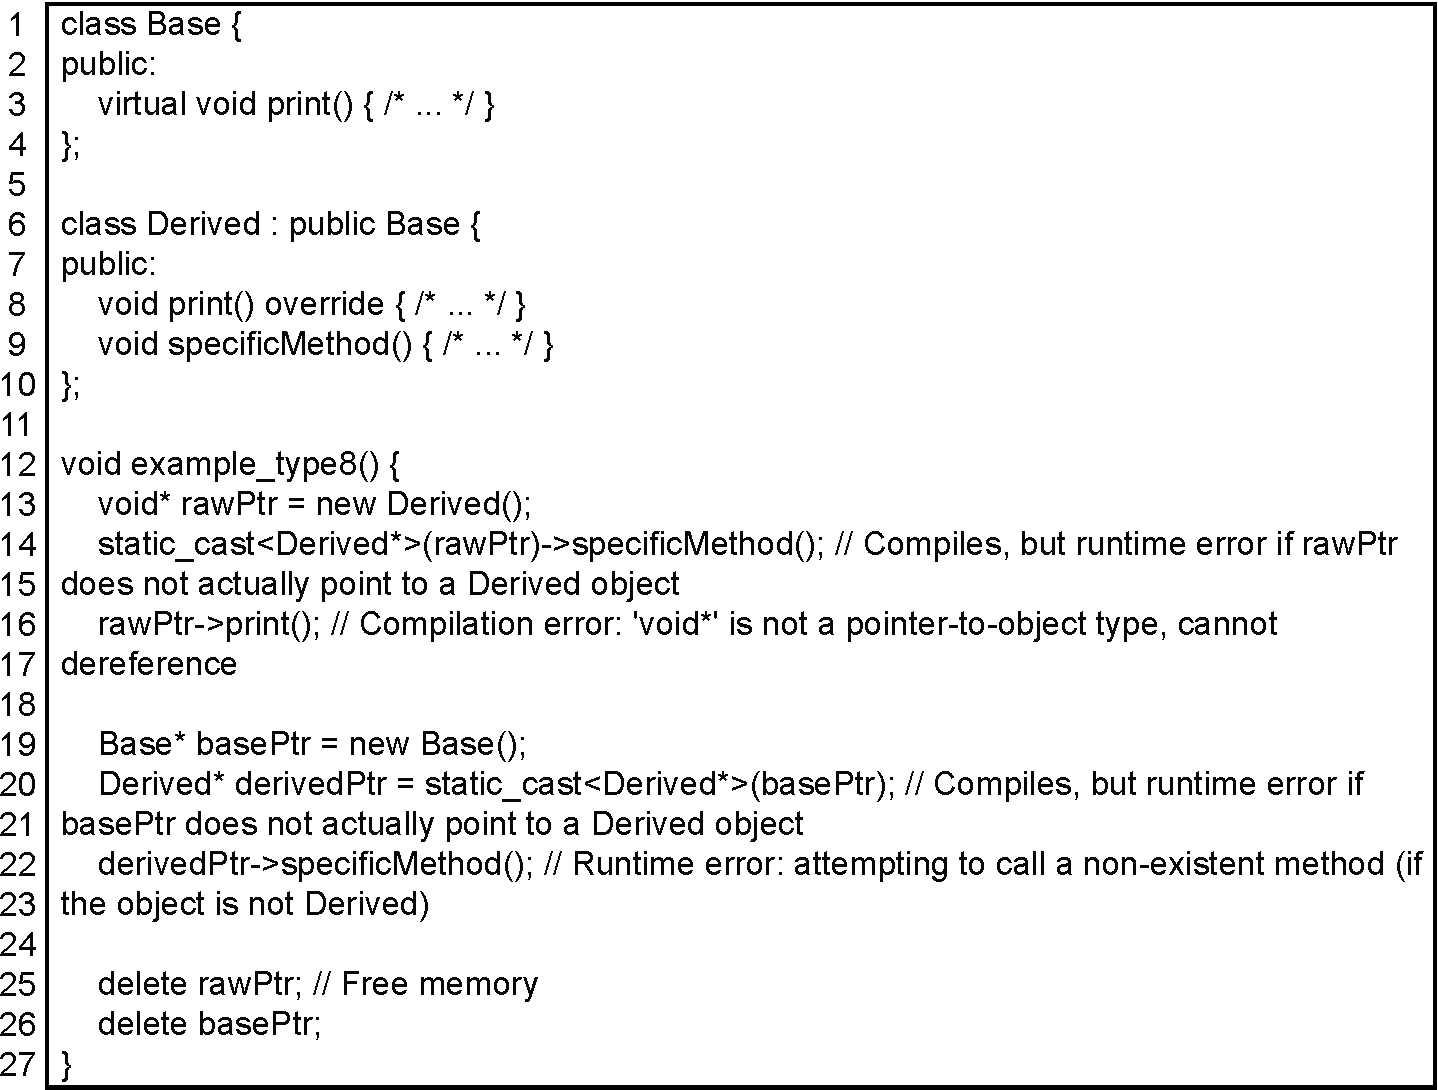
\includegraphics[width=0.5\textwidth]{pdf/Codes/Code6.pdf}
\end{figure}
\subsubsection{Referencing non-existent classes}
This error type refers to the code referencing a class that is not defined in the C++ standard library, project dependencies, or the current codebase. This is usually because the translation directly copied Java-specific libraries, and these classes do not have direct corresponding implementations in C++, requiring the use of different libraries or design patterns as alternatives.
\begin{figure}[H]
  \centering
  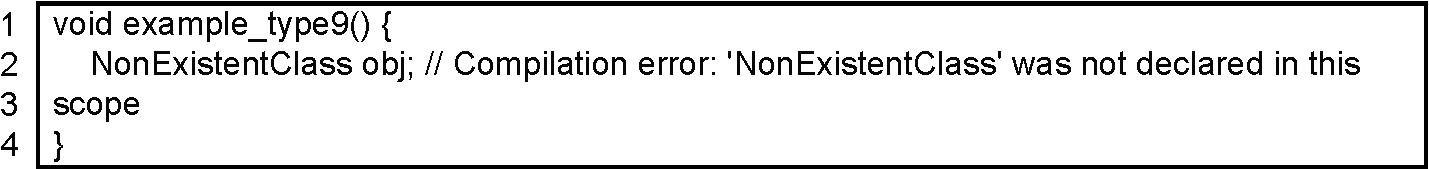
\includegraphics[width=0.5\textwidth]{pdf/Codes/Code7.pdf}
\end{figure}
\subsubsection{Method partially unimplemented (partially missing)}
Unlike "Method not implemented (entirely missing)", this error type refers to methods that have an implementation body, but their internal logic is incomplete, contains placeholders, or is severely simplified, failing to achieve the full functionality of the original Java code.
\begin{figure}[H]
  \centering
  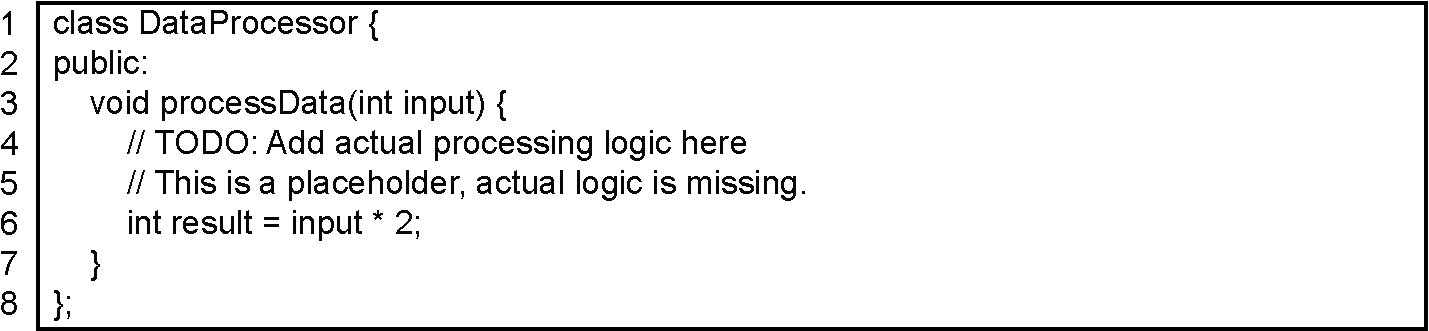
\includegraphics[width=0.5\textwidth]{pdf/Codes/Code8.pdf}
\end{figure}
\subsubsection{Improper memory management}
This error type specifically targets C++'s manual memory management mechanism. It primarily includes memory leaks, double-freeing the same memory block, or using dangling pointers that have been freed.
\begin{figure}[H]
  \centering
  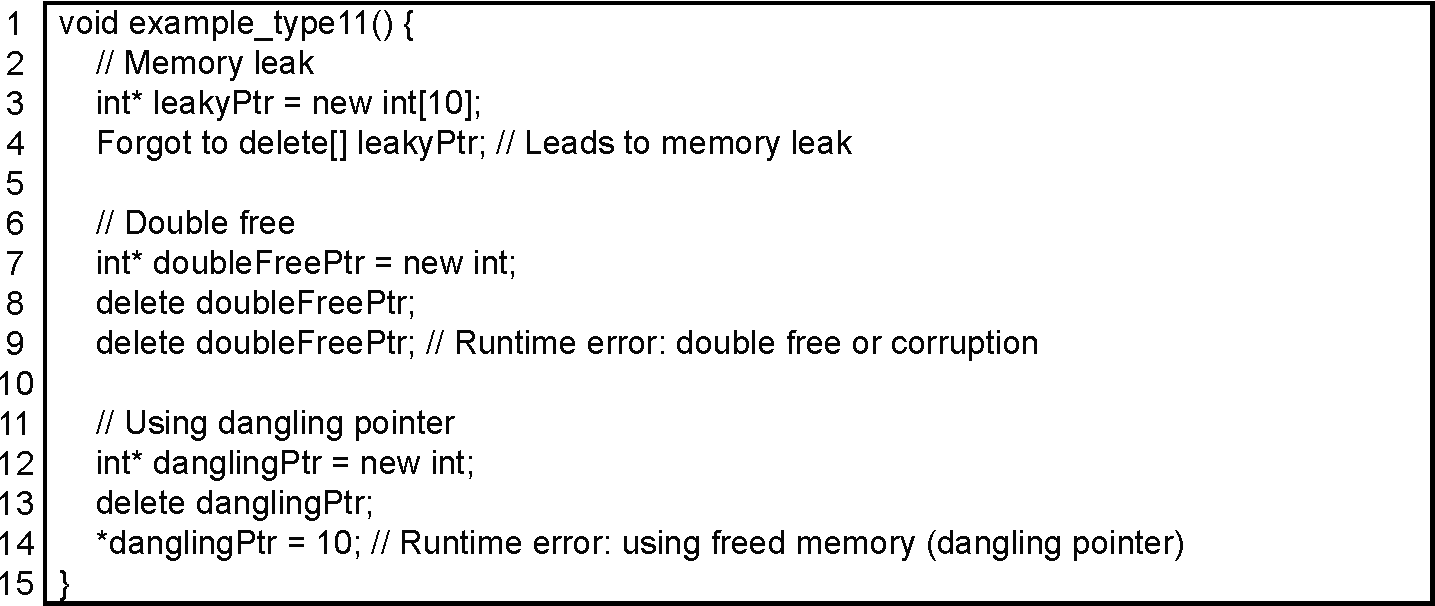
\includegraphics[width=0.5\textwidth]{pdf/Codes/Code9.pdf}
\end{figure}

\begin{table*}[htbp]
  \centering
  \caption{Error Types}
  \label{tab:error-types}
  \begin{tabularx}{\textwidth}{XXX}
    \hline
    \textbf{Error Type} & \textbf{Entity} & \textbf{Description} \\
    \hline
    Referencing non-existent methods or member variables & Method Call / Member Access & Calling a method or accessing a member variable that does not exist in a class or its base class. \\
    Parameter list mismatch & Method Declaration & The parameters provided in a function call do not match the quantity, type, or order of any available overloaded version of that function. \\
    Missing header file & \#include Directive & The code uses a class, function, or macro but fails to include the corresponding header file, leading to a compilation failure. \\
    Method not implemented (entirely missing) & Method Definition & A member function is declared, but no implementation is provided for it, or the implementation body is empty. \\
    Variable initialization/usage error & Variable Declaration / Constructor & Failure to initialize reference or constant members in a constructor's initializer list, or using any variable before it has been initialized. \\
    Incorrect pointer usage & Pointer Operation & Improper operations on C++ pointers, such as dereferencing a void pointer or performing incorrect type conversions. \\
    Referencing non-existent classes & Class Reference / Type Usage & The code references a class that is not defined in the standard library, project dependencies, or the current codebase. \\
    Method partially unimplemented (partially missing) & Method Implementation & The method has an implementation body, but its internal logic is incomplete, contains placeholders, or is simplified, failing to match the original functionality. \\
    Improper memory management & Memory Allocation/Deallocation & Errors related to manual memory management, including memory leaks, double-freeing memory, or using dangling pointers. \\
    \hline
  \end{tabularx}
\end{table*}

\subsection{Overall Performance}
\subsubsection{Overall Correctness Rate/Error Rate}
Across all evaluated LLMs (GPT and DeepSeek), a total of 1994 distinct methods were translated and analyzed. Of these, 1211 methods were accurately translated, while 783 methods contained one or more identified errors. The overall correctness rate was 60.73\%, and the error rate was 39.27\%. This data establishes a baseline reference for LLM performance in Java to C++ code translation.

\begin{table}[H]
  \centering
  \label{tab:translation-stats}
  \begin{tabular}{lrr}
    \hline
    Metric                         & Quantity & Proportion (\%) \\
    \hline
    Correctly Translated Methods   & 1211     & 60.73           \\
    Incorrectly Translated Methods & 783     & 39.27           \\
    \hline
  \end{tabular}
\end{table}

Based on data analysis, a significant portion of methods were accurately translated, though a notable percentage contained identified errors. These findings are important for understanding current LLM proficiency in cross-language code conversion and provide reference points for future advancements.

\subsubsection{Performance w.r.t LLMs.}
Based on existing translation results, we can compare the overall translation efficiency of GPT and DeepSeek.
\begin{itemize}[leftmargin=1.5em]
    \item \textbf{GPT: }GPT processed a total of 1099 methods. Of these, 614 methods were correctly translated, and 485 methods were incorrectly translated. This gives GPT an overall correctness rate of 55.87\%.
    \item \textbf{DeepSeek: }DeepSeek processed a total of 895 methods. It completed 597 correct translations and 298 incorrect translations. This gives DeepSeek a higher overall correctness rate of 66.70\%.
\end{itemize}

\begin{figure}[H]
  \centering
  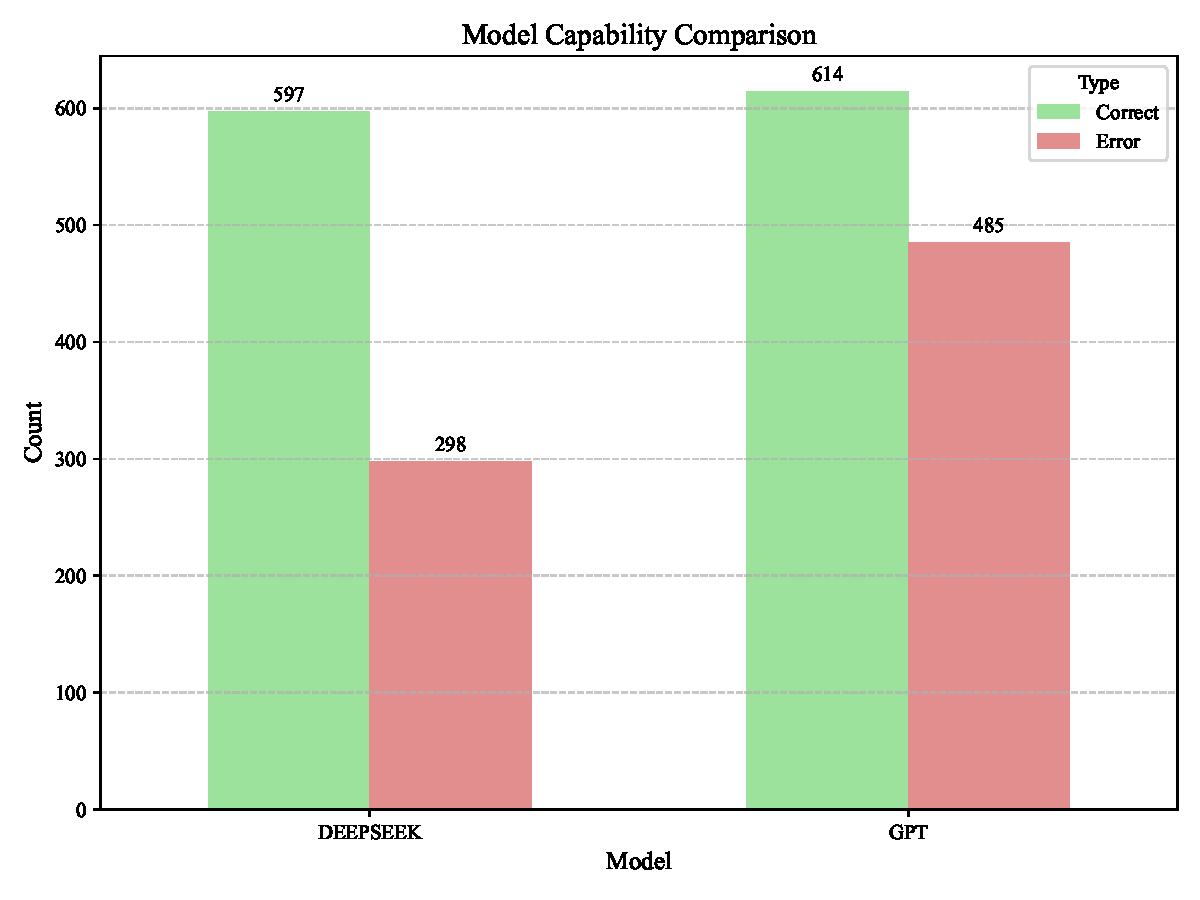
\includegraphics[width=0.5\textwidth]{pdf/Model Capability Comparison.pdf}
\end{figure}


DeepSeek’s overall correctness rate (66.70\%) was significantly higher than GPT’s (55.87\%), demonstrating an absolute advantage of 10.83 percentage points. This indicates that, in this experimental setup, for the methods it completed, DeepSeek was, on average, more reliable in generating correct Java to C++ translations.

\subsubsection{Performance w.r.t Projects.}
To investigate how project characteristics affect translation performance, we conducted a comparative analysis of the translation results across five different projects. The table below summarizes the correctness rate and error distribution for each project under the class strategy.

\begin{table*}[]
  \centering
  \begin{tabularx}{\textwidth}{XXXXXX}
    \hline
    Project Name & File Count & Correct Methods & Erroneous Methods & Correctness Rate &  Dominant Error Types (Count) \\
    \hline
    Cookie & 9 & 166 & 26 & 86.5\% & Missing header file(6), Improper memory management(4) \\
    EnableJUnit4MigrationSupport & 32 & 293 & 334 & 46.7\% & Method not implemented (entirely missing)(224), Referencing non-existent classes(55) \\
    HoverMenuService & 9 & 58 & 50 & 53.7\% & Method not implemented (entirely missing)(44) \\
    IntMath & 7 & 89 & 97 & 47.8\% & Method not implemented (entirely missing)(91) \\
    NoopIndexDAO & 21 & 609 & 264 & 69.8\% & Method not implemented (entirely missing)(253) \\
    \hline
  \end{tabularx}
\end{table*}

Based on the data, the EnableJUnit4MigrationSupport project, which has the highest file count (32), also exhibits nearly the lowest correctness rate (46.7\%). This preliminarily suggests that as project scale increases, contextual dependencies may become more complex, leading LLMs to make more errors during holistic class-level translation, particularly generating a large number of "Method not implemented (entirely missing)" and "Referencing non-existent classes" errors. Similarly, the second-largest project, NoopIndexDAO, while having a decent correctness rate (69.8\%), also suffers from a high volume of "Method not implemented (entirely missing)" errors.

Although the IntMath project has the fewest files (7), its translation correctness rate is also very low (47.8\%), with errors almost entirely concentrated in "Method not implemented (entirely missing)" (accounting for 93.8\% of its total errors). This may imply that the project involves numerous Java-specific design patterns and libraries, as well as fundamental differences from C++ in memory management, null handling, and standard library functionalities. When faced with methods requiring cross-language paradigm shifts and idiomatic C++ implementations, LLMs struggle to find direct correspondences, thus tending to omit their implementation.

The Cookie project stands out with the highest correctness rate of 86.5\%. As a smaller-scale project (9 files), its error types are also more dispersed, without a single error type being overwhelmingly dominant. This might indicate that the project's code structure is relatively simple with clear dependencies, making it more suitable for LLM translation.

In summary, under the class strategy, project scale and content complexity are key factors influencing translation quality. For large-scale or logically complex projects, LLMs struggle to maintain a complete contextual understanding, leading them to frequently omit method implementations, which severely impacts the completeness and usability of the code.


\subsubsection{Error Type Distribution}
Analyzing and comparing the distribution of all identified error types across the entire translation corpus, we observed that certain hallucination categories predominated. "Method not implemented (entirely missing)" was the most prevalent, accounting for a total of 624 instances. This single error type constituted approximately 51.53\% of all identified errors, revealing the current LLMs' inadequacy in generating complete code structures.

Other significant error types include:
\begin{itemize}[leftmargin=1.5em]
    \item \textbf{Referencing non-existent classes: }This category accounted for 61 instances. This type primarily arises from LLMs using non-existent classes in C++ when generating translated files. These may stem from differences between Java and C++ or be entirely a product of LLM hallucination. This error indicates that LLMs still struggle with correctly identifying or hallucinating external class dependencies.
    \item \textbf{Referencing non-existent methods or member variables: }36 instances. This error indicates difficulty in maintaining member access consistency within classes.
    \item \textbf{Method partially unimplemented (partially missing): }This error type occurred 21 times, indicating cases where a method was generated but not completed.
\end{itemize}

Other less common but still noteworthy error types included "Missing header file" (13 instances) and "Parameter list mismatch" (11 instances).
\begin{figure}[H]
  \centering
  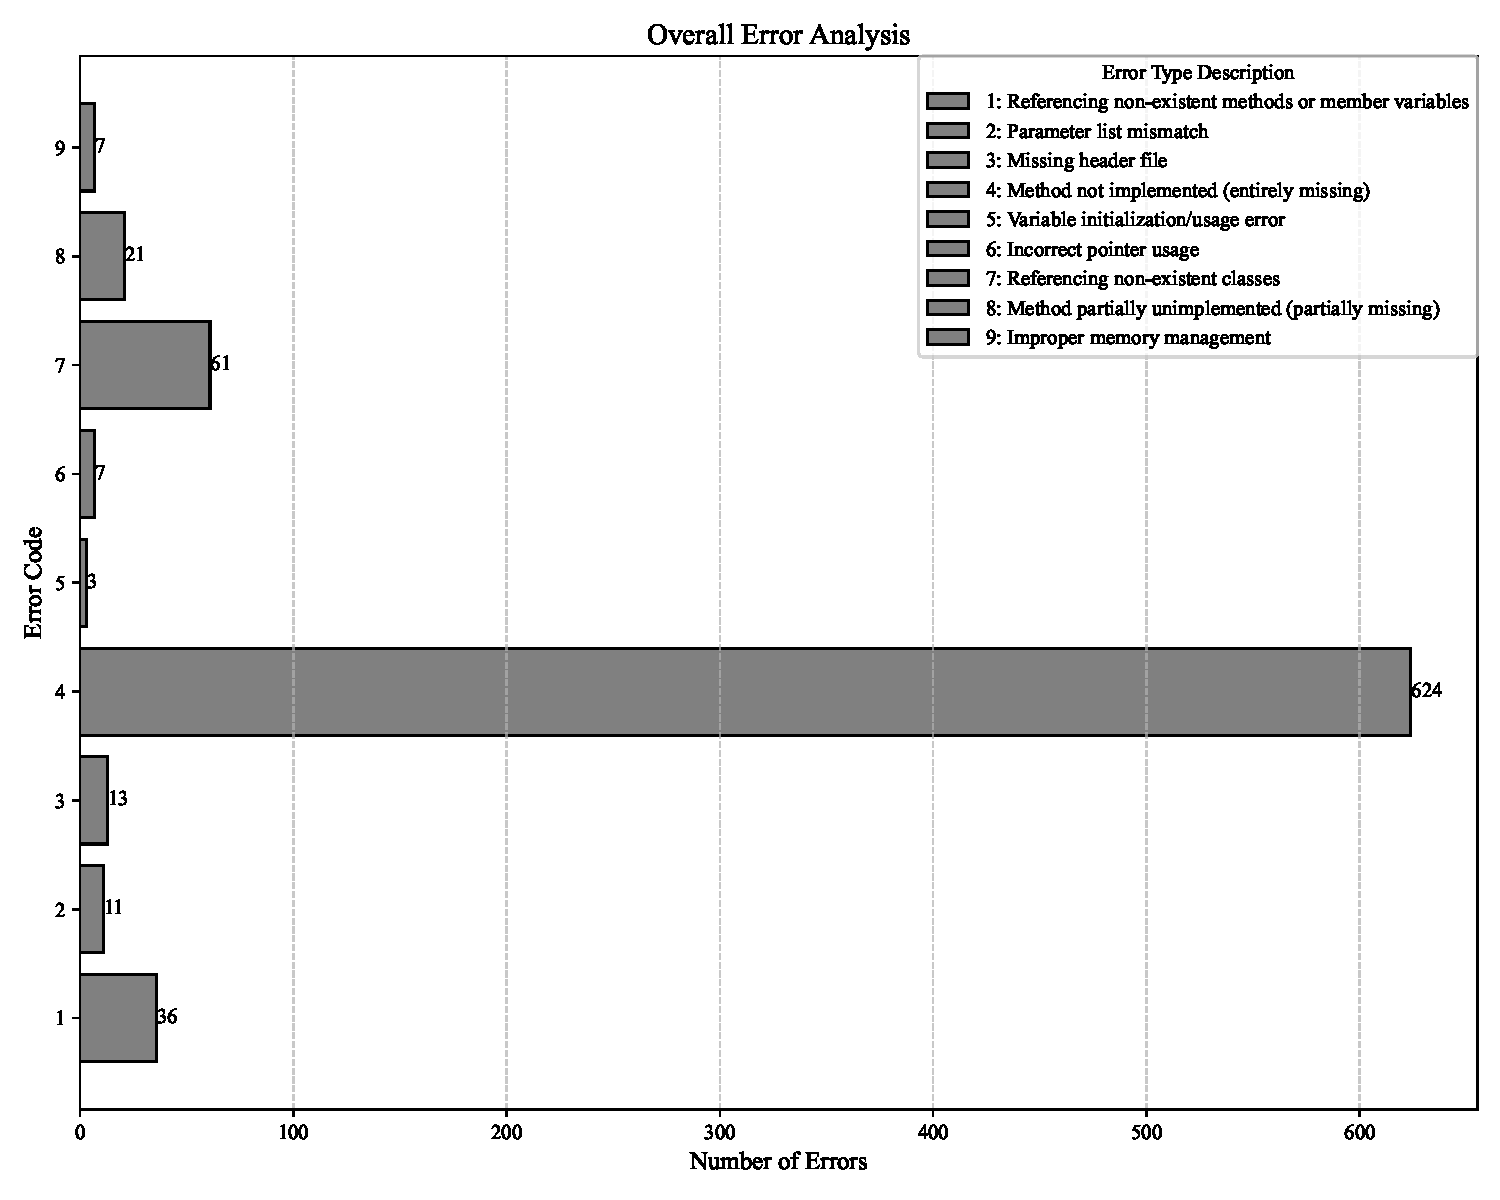
\includegraphics[width=0.5\textwidth]{pdf/Overall Error Analysis.pdf}
\end{figure}

The overwhelming dominance of “Method not implemented (entirely missing)” is not just a quantitative finding but also qualitatively highlights fundamental limitations of LLMs. This suggests that when faced with complex class translation tasks, LLMs often opt to omit entire methods rather than attempting to translate them. This also points to a structural hallucination, where the model completely fails to produce the expected output, rather than merely generating semantically or syntactically incorrect code.

If LLMs frequently omit entire methods, it implies significant challenges in maintaining long-term coherence and completeness in medium to large-scale code projects. The occurrence of this error may stem from several factors: First, the LLM's context window might be insufficient to accommodate the entire class definition and its dependencies, preventing a complete analysis of methods and leading to the omission of their entire implementation. Second, when target methods are not explicitly referenced or prompts are too broad, LLMs may fail to fully grasp the implicit requirements of all methods within the translated class. Finally, in situations of high uncertainty or perceived complexity, LLMs struggle to fully convert Java language features to C++. They might choose to omit or fill with TODOs for later completion rather than generating highly erroneous or uncompilable code. This type of hallucination is particularly critical as it results in incomplete or non-functional target code, requiring substantial manual intervention.

The high incidence of method omission suggests that, without explicit, fine-grained guidance, current LLMs may lack an internal coherent understanding of software project structure and code completeness, making them less adept at automating large, multi-component code migration tasks. While they excel at generating syntactically plausible code snippets, their ability to generate complete, coherent, and functionally equivalent project systems remains nascent. To complete the translation and migration of an entire project, LLMs need to understand the complete structure of the target code, not just the internal logic of individual methods. Future LLM development needs to focus on improving their ability to understand code as a structured system, rather than merely translating raw code as a series of independent fragments.


\subsubsection{Error Type Distribution by Model}
A detailed examination of the error type distribution for each model reveals different characteristics in their hallucination frequencies.
%\begin{figure}[H]
%  \centering
%  
\includegraphics[width=0.5\textwidth]{Class_Method_Error_Type_Stacked_Bar_Chart.pdf}
%\end{figure}

\begin{itemize}[leftmargin=1.5em]
    \item \textbf{GPT Error Distribution: }GPT's most common error was "Method not implemented (entirely missing)," with 373 instances. Other significant errors included "Referencing non-existent classes" (41 instances) and "Referencing non-existent methods or member variables" (28 instances).
    \item \textbf{DeepSeek Error Distribution: }For DeepSeek, "Method not implemented (entirely missing)" was also the most common error, but its count was significantly lower than GPT's, at 251 instances. Other errors included "Referencing non-existent classes" (20 instances) and "Referencing non-existent methods or member variables" (8 instances).
\end{itemize}

\begin{figure}[H]
  \centering
  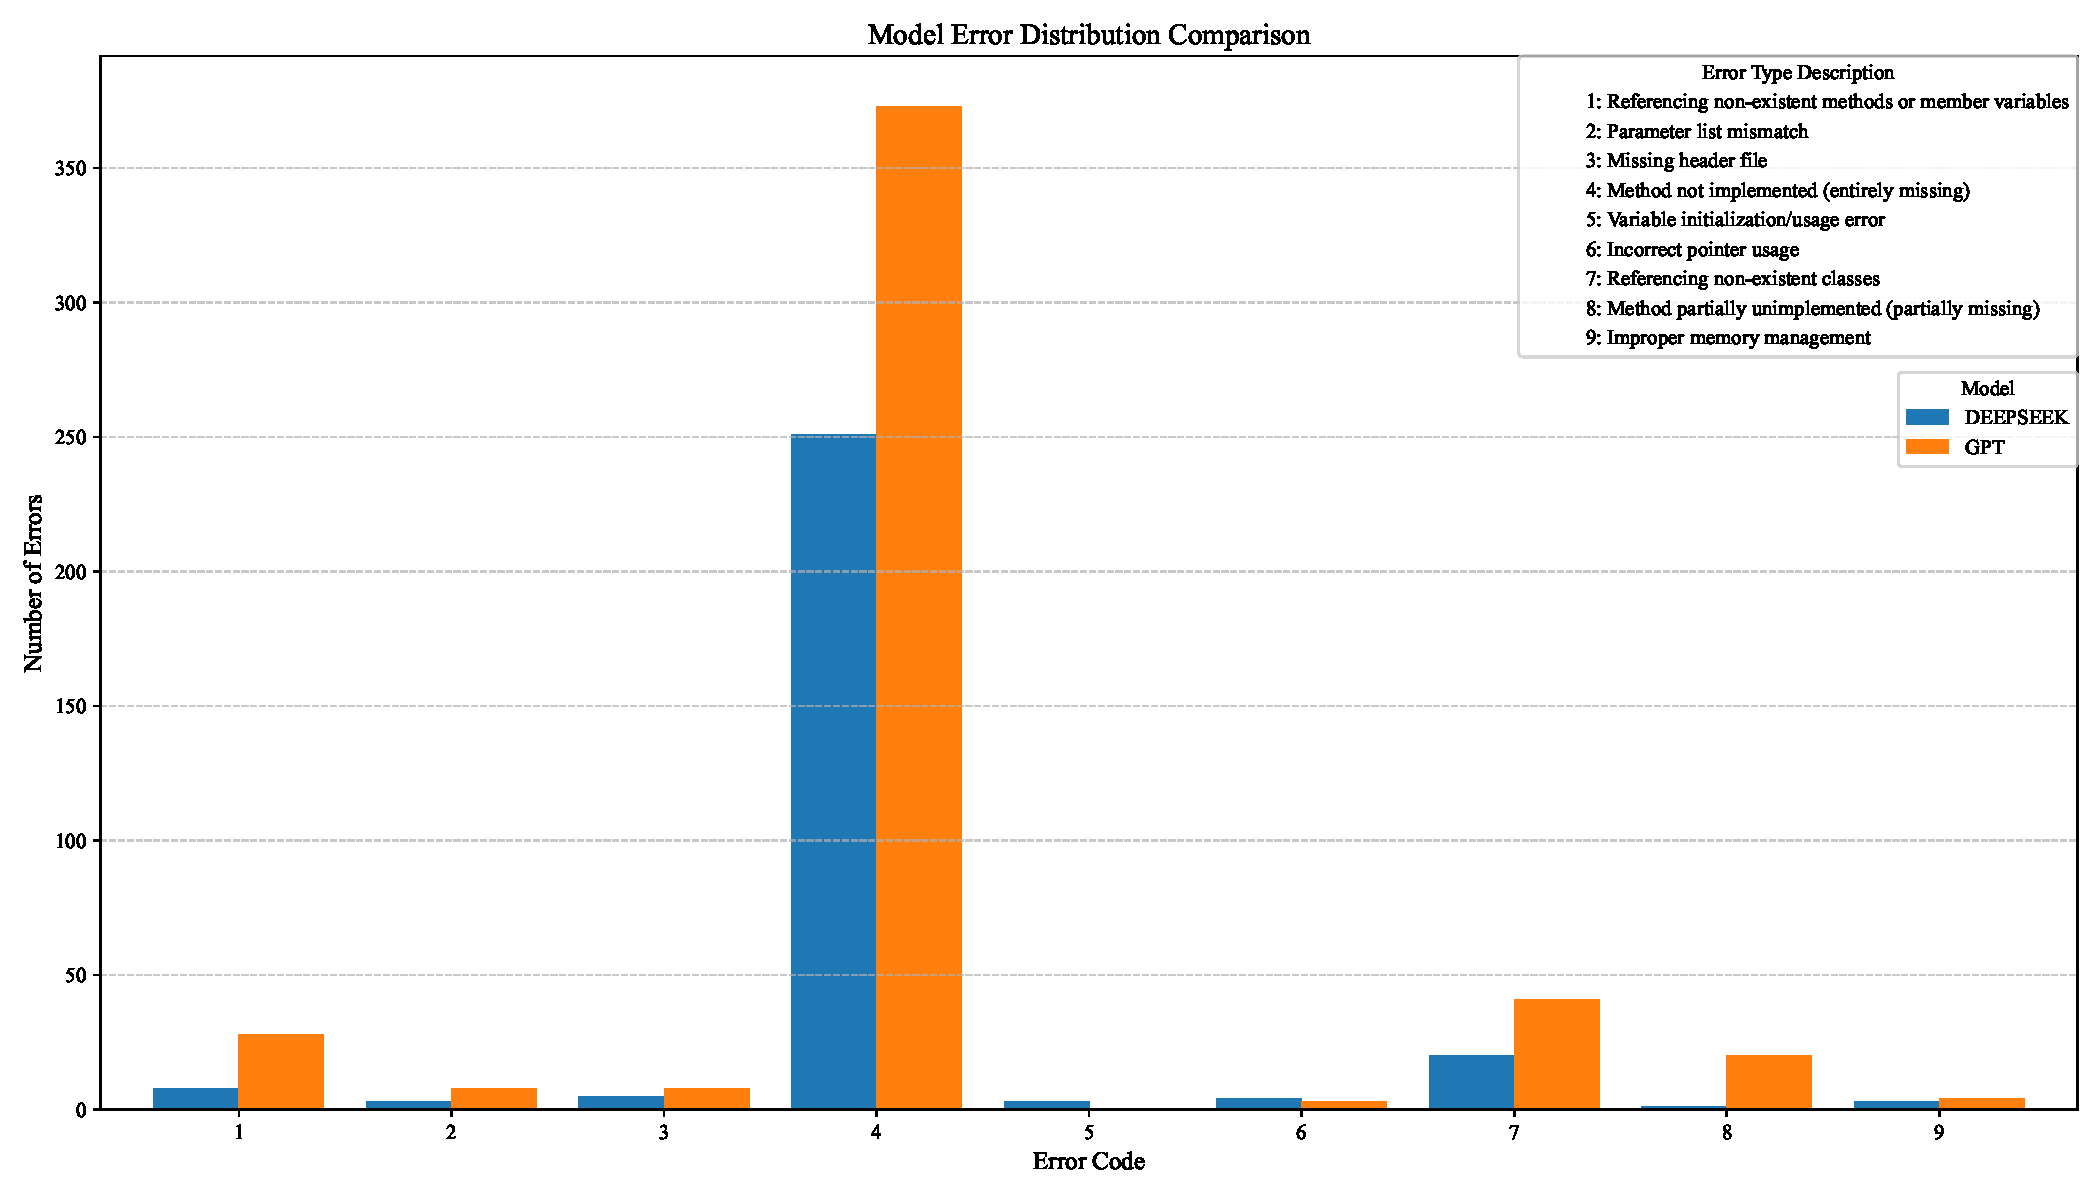
\includegraphics[width=0.5\textwidth]{pdf/Model Error Distribution Comparison.pdf}
\end{figure}

DeepSeek demonstrated a stronger ability to prevent complete method omissions, with 122 fewer "Method not implemented (entirely missing)" errors than GPT. This factor contributed to DeepSeek's higher overall correctness rate.DeepSeek in code translation accuracy and completeness showed a clear advantage, especially in avoiding "Method not implemented" and "Referencing non-existent" errors. GPT in this type of basic translation method appears to have a higher error rate, especially in generating complete method implementations. If the main goal is to efficiently obtain compilable and functionally correct translated code, then DeepSeek seems to be the preferred choice.

\subsection{Data Analysis Summary}

\begin{itemize}[leftmargin=1.5em]
    \item \textbf{Pervasive Hallucinations: }Large Language Models (LLMs), including GPT and DeepSeek, exhibit a significant hallucination rate in Java to C++ code translation. The most prevalent and impactful error type is "Method not implemented (entirely missing)." This phenomenon indicates a deficiency in LLMs' ability to fully comprehend code project structures and migrate complete code.
    \item \textbf{Model-Specific Strengths: }DeepSeek generally outperformed GPT in overall correctness, primarily due to its lower rate of "Method not implemented" errors, revealing DeepSeek's stronger inherent ability to maintain code completeness.
\end{itemize}


